% Created: Enze Chen, August 2017

% Chapter 7 of the MSE 142 coursereader.
% This chapter continues the discussion from last chapter by extending into introductory quantum field theory.
% We start with second quantization and then move on to deriving the Casimir force. 
% We conclude with a brief discussion of phonons.

% Uncomment the following three lines and last line to individually compile this chapter
%\documentclass[12pt, english]{book}
%\usepackage{142crstyle}
%\begin{document}

\chapter{Quantum Field Theory} \label{ch:qft}
%{ \doublespacing 
One of the greatest challenges facing scientists of the 20$^{\text{th}}$ century was using quantum mechanics to accurately model the behavior of subatomic particles, which usually involved painstakingly reconciling quantum mechanics with special relativity. 
Eventually, they developed the framework of quantum field theory (QFT), which treats particles as excited states (quanta) of the underlying \emph{field} (hence the name).\footnote{For an interesting explanation with helpful diagrams, see \href{https://www.ribbonfarm.com/2015/08/20/qft/}{this post} from Brian Skinner.} 
We can think of a field as a network of interconnected balls and springs and the strength of the field can be measured by the amount of displacement from rest. 
In this chapter, we will only scratch the surface of QFT as we explore some of its most surprising and most important results. 


% % % % % % % % % % % % % % % % % % % % % % % % % % % % % % % % % % % % % 
% % % % % % % % % % % % % % % % % % % % % % % % % % % % % % % % % % % % % 
% % % % % % % % % % % % % % % % % % % % % % % % % % % % % % % % % % % % %
\section{Second quantization}

So far, all of the systems we have analyzed fall into the category of \textbf{first quantization}, where we describe a quantum mechanical system by its wavefunction and we describe its surroundings (e.g., the potential well) using classical mechanics. 
While this formulation is well-defined for a single-particle system, many of its expressions grow combinatorially unwieldy for many-particle systems. 
In QFT, we are less concerned with the behavior of individual particles (``Which state is particle $i$ in?") and we're more interested in the overall distribution (``How many particles are in state $\ket{\alpha}$?"). 
This calls for \textbf{second quantization}, which places a QHO at each point in space such that the strength of the field is quantized. 


% % % % % % % % % % % % % % % % % % % % % % % % % % % % % % % % % % % % % 
% % % % % % % % % % % % % % % % % % % % % % % % % % % % % % % % % % % % %
\subsection{Occupation number operator}

Recall that for single particles, we used bra-ket notation to represent the quantum state as $\ket{\alpha}$, where $\alpha = 0,\ 1,\ 2,\ \dots$. 
Now we will define the \textbf{occupation number operator} $\hat{n}_{\alpha}$ to be the number of particles in the single-particle state $\ket{\alpha}$. 
These occupation numbers label the basis state, which is represented as

\begin{tcolorbox} [title=Basis vector] \vspace{-2ex}
	\begin{equation}
		\ket{\Psi} = \ket{\hat{n}_0,\ \hat{n}_1,\ \hat{n}_2,\ \dots,\ \hat{n}_{\alpha},\ \dots} \label{eq:fock}
	\end{equation}
\end{tcolorbox} 

For bosons, $\hat{n}_{\alpha}$ can be any non-negative integer, while for fermions $\hat{n}_{\alpha}$ must be 0 or 1.\footnote{Bosons are a class of subatomic particles that have integer spins (e.g. photons, gluons, and other force carriers), while fermions are another class of subatomic particles that have non-integer spins (e.g. electrons) and obey the Pauli exclusion principle.} 
This formalism allows us to treat the quantum system as an ensemble of indistinguishable particles. 
The total number of particles is then

\begin{equation}
	\hat{N} = \sum_{\alpha} \hat{n}_{\alpha}
\end{equation}

\noindent which sums all the particles in all the states.

To get a better understanding of the basis vectors, let's consider some special cases. 
First, there is a \textbf{vacuum state} with no particles represented as

\begin{equation}
	\ket{0} = \ket{0,\ 0,\ 0,\ \dots}
\end{equation}

The single-particle state that we've previously encountered can be written as

\begin{equation}
	\ket{1_{\alpha}} = \ket{0,\ 0,\ \dots, 1_{\alpha},\ \dots} = \psi_{\alpha}
\end{equation}

From this point, many-particle, many-state bases can be deduced, and we'll leave it as an exercise to the reader to find the proper normalization coefficient.

Noticeably, the basis vector we defined in \autoref{eq:fock} does not have a fixed particle number. 
This allows us to introduce and take away particles from our quantum mechanical system, which is conveniently handled by the creation and annihilation operators.


% % % % % % % % % % % % % % % % % % % % % % % % % % % % % % % % % % % % % 
% % % % % % % % % % % % % % % % % % % % % % % % % % % % % % % % % % % % %
\subsection{Creation and annihilation operators}

In the previous chapter, we used the creation and annihilation operators to arrive at different energy states of the quantum harmonic oscillator. 
Here, since we are dealing with an ensemble of many particles in many states, we will have a different $\ad_{\alpha}$ and $a_{\alpha}$ for each state $\ket{\alpha}$. 
Furthermore, the definition of the operators has changed, and now the creation operator acts as if it's truly ``creating" another particle and adding it to the system. 
Formally, we have

\begin{equation}
	\ad_{\alpha} \ket{\hat{n}_1,\ \hat{n}_2,\ \dots,\ \hat{n}_{\alpha},\ \dots} = \sqrt{\hat{n}_{\alpha}+1}\ket{\hat{n}_1,\ \hat{n}_2,\ \dots,\ \hat{n}_{\alpha}+1,\ \dots}
\end{equation} 

Similarly, we define the annihilation operator as

\begin{equation}
a_{\alpha} \ket{\hat{n}_1,\ \hat{n}_2,\ \dots,\ \hat{n}_{\alpha},\ \dots} = \sqrt{\hat{n}_{\alpha}}\ket{\hat{n}_1,\ \hat{n}_2,\ \dots,\ \hat{n}_{\alpha}-1,\ \dots}
\end{equation} 

A demonstration of the creation operator would be to apply it to the vacuum state to obtain the single-particle state:

\begin{equation}
	\ad_{\alpha} \ket{0} = \ket{1_{\alpha}}
\end{equation}

Likewise, if we apply the annihilation operator to the vacuum state, or any basis vector with zero particles in the particular state, we get zero.

\begin{equation}
	a_{\alpha} \ket{0} = 0, \qquad a_{\alpha} \ket{\hat{n}_1,\ \dots,\ \hat{n}_{\alpha}=0,\ \hat{n}_{\beta},\ \dots} = 0
\end{equation}

If we apply the annihilation operator and creation operator in succession, we obtain

\begin{equation*}
\ad_{\alpha} a_{\alpha} \ket{\hat{n}_1,\ \hat{n}_2,\ \dots,\ \hat{n}_{\alpha},\ \dots} = \hat{n}_{\alpha}\ket{\hat{n}_1,\ \hat{n}_2,\ \dots,\ \hat{n}_{\alpha},\ \dots}
\end{equation*}

\noindent which gives the relation

\begin{equation}
	\hat{n}_{\alpha} = \ad_{\alpha}a_{\alpha}
\end{equation}

This is similar to what we saw with the QHO and is another definition for the number operator. 
We will also state the commutation relations here without proof for two arbitrary states $\alpha$ and $\beta$. 
Note that these are the same commutation relations as the QHO, and it's perfectly valid in QFT to consider bosons as energy quanta of an underlying field of quantum oscillators.

\begin{equation}
	\left[\ad_{\alpha},\ad_{\beta}\right] = \left[a_{\alpha},a_{\beta}\right] = 0, \qquad \left[a_{\alpha}, \ad_{\beta}\right] = \delta_{\alpha,\beta}
\end{equation}

With the formal definitions of second quantization out of the way, we can proceed to a more interesting analysis. 
Since we have an operator that gives the number of particles of each state in our system, we can find the total energy of all the particles by a conventional summation. 
The expression for the Hamiltonian becomes

\begin{equation}
	\hat{H} = \sum_{\alpha} \hbar\omega_{\alpha} \left(\hat{n}_{\alpha} + \frac{1}{2} \right) = \sum_{\alpha} \hbar\omega_{\alpha} \left(\ad_{\alpha}a_{\alpha} + \frac{1}{2}\right)
\end{equation}

Here we give each quantum state its individual frequency $\omega_{\alpha}$. 
Now, as we showed in the last chapter, the Hamiltonian is a Hermitian operator, which means it should return a sensible value for the expectation. 
If we find the expected total energy of the vacuum state, we get the following:

\begin{align*}
	\mel{0}{\hat{H}}{0} &= \sum_{\alpha} \hbar\omega_{\alpha} \cancelto{0}{\mel{0}{\ad_{\alpha}a_{\alpha}}{0}} + \sum_{\alpha}\hbar\omega_{\alpha}\left(\frac{1}{2}\right) \\
	&= \sum_{\alpha} \frac{\hbar\omega_{\alpha}}{2} \longrightarrow \infty
\end{align*}

In the second line, the summation of zero-point energies over an unbounded number of possible states seemingly gives infinite energy from vacuum fluctuations alone. 
Crazy! 
One of the early results of QFT was that the underlying field is in constant flux and it has physically relevant consequences. 
We'll see in the next section how we might resolve this ``infinite energy" to make it physically interpretable.


% % % % % % % % % % % % % % % % % % % % % % % % % % % % % % % % % % % % % 
% % % % % % % % % % % % % % % % % % % % % % % % % % % % % % % % % % % % %
% % % % % % % % % % % % % % % % % % % % % % % % % % % % % % % % % % % % %
\section{Quantum electrodynamics}

One of the crowning achievements of QFT is the construction of \textbf{quantum electrodynamics} (QED), which describes how light and matter interact in the quantized electromagnetic field.\footnote{For a friendlier introduction to QED, see R. P. Feynman, \href{https://en.wikipedia.org/wiki/QED:_The_Strange_Theory_of_Light_and_Matter}{\emph{QED: The Strange Theory of Light and Matter}}, 1985.} 
QED was the first theory to reconcile quantum mechanics and special relativity, and it led to extremely accurate calculations for the Lamb shift,\footnote{A good description of the Lamb shift is provided by \href{http://hyperphysics.phy-astr.gsu.edu/hbase/quantum/lamb.html}{Rod Nave}.} spontaneous emission (discussed in the next chapter), and a mysterious phenomenon called the Casimir effect, which we will discuss here. 
As it turns out, all of these phenomenon can be explained by the vacuum fluctuation energy and the way it interacts with matter.

\begin{figure}[!h]
	\centering
	\subfloat[]{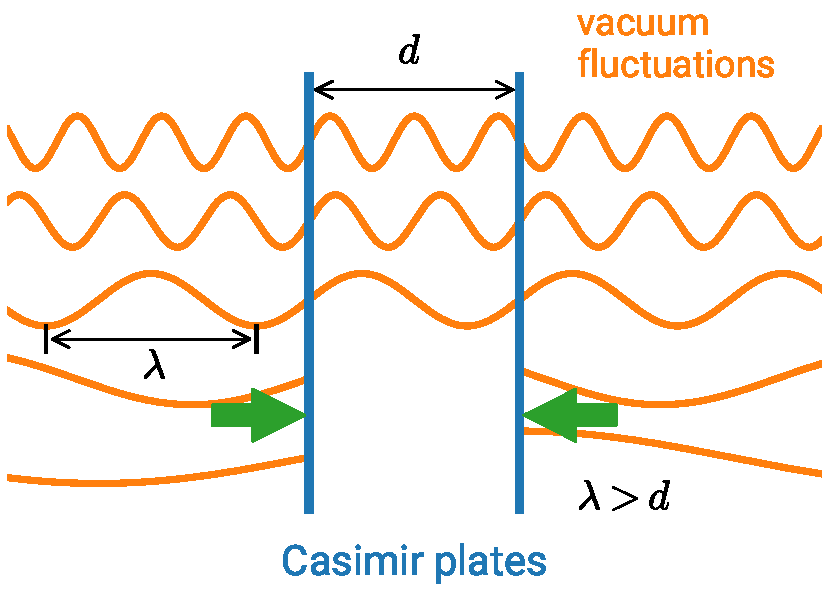
\includegraphics[width=0.5\linewidth]{casimir.pdf} \label{fig:casimir-fig}} \hspace{2ex}
	\subfloat[]{\includegraphics[width=0.45\linewidth]{casimir-exp.png} \label{fig:casimir-exp}}
	\caption{\protect\subref{fig:casimir-fig} A schematic of the Casimir effect observed between two metal plates. 
	The boundary conditions at the plates allow a limited number of standing waves to exist in the middle region, which is fewer than the amount of vacuum fluctuations outside the plates. 
	This creates a pressure difference that forces the plates together. 
	\protect\subref{fig:casimir-exp} An experimental measurement using an atomic force microscope of the Casimir force between an Al-coated sphere and an Al-coated surface. 
	Reproduced from U. Mohideen and A. Roy, \href{https://journals.aps.org/prl/abstract/10.1103/PhysRevLett.81.4549}{\emph{Phys. Rev. Lett.}} 81, 1998.}
	\label{fig:casimir}
\end{figure}


% % % % % % % % % % % % % % % % % % % % % % % % % % % % % % % % % % % % %
% % % % % % % % % % % % % % % % % % % % % % % % % % % % % % % % % % % % %
\subsection{Casimir effect}

In 1948, Dutch physicist Hendrik Casimir predicted that the zero-point energy in the QED vacuum could cause a physical force between two neutral conducting plates.\footnote{H. B. G. Casimir, \href{http://www.dwc.knaw.nl/DL/publications/PU00018547.pdf}{\emph{Proc. Kon. Ned. Akad. Wetensch.}} 51, 1948.} 
This phenomenon became known as the \textbf{Casimir effect} (\autoref{fig:casimir}) and can be explained using QED and second quantization. 
Although there are infinite vacuum fluctuations in the space outside of the plates, the reflective surface of the plates actually exclude virtual photons (manifestations of the underlying electromagnetic field) with wavelengths longer than the interplanar distance. 
Essentially you can think of the plates as nodes for the wave-like photons, so only wavelengths that line up perfectly will remain in the middle region. 
This reduces the energy density between the two plates, and much like normal pressure, the Casimir force pushes the two plates closer together.

Since we should not be merely satisfied with a description, let's try to find an analytical argument and really derive the strength of this Casimir force. 
Since we are working with the QED vacuum, we have to first establish the \textbf{dispersion relation} for photons, which gives the relationship between the frequency and the wave number. 
Mathematically, this is written as

\begin{tcolorbox}[title=Dispersion relation] \vspace{-2ex}
	\begin{equation}
		\omega_n = ck_n \label{eq:dispersion}
	\end{equation}
\end{tcolorbox}

\noindent where $c$ is the speed of light and $k_n = n \pi / d$. 
We also make use of the subscript $n$ here to index individual solutions, just like we did with the particle in a box. 


% % % % % % % % % % % % % % % % % % % % % % % % % % % % % % % % % % % % %
% % % % % % % % % % % % % % % % % % % % % % % % % % % % % % % % % % % % %
\subsection{Regularization and renormalization}

Now we will try to find the amount of energy in between the two plates and subtract that quantity from the energy on the outside, and that should give us quantitative information about the Casimir force (its derivative will, anyways). 
Inside the two conducting plates, we have the following expression for the total energy:

\begin{align*}
	E_{\text{in}} &= \sum_{\alpha} \frac{\hbar\omega_{\alpha}}{2} \\
	&= \sum_{n=0}^{\infty} \frac{\hbar c k_n}{2} \\
	&= \frac{\hbar \pi c}{2d} \sum_{n=1}^{\infty} n \numberthis \label{eq:casimir-in}
\end{align*}

We use a discrete sum for the discrete energy levels of the bound photons, and just like before, we see that the total energy approaches infinity. 
Now, those of you that have taken complex analysis\footnote{Which I expect to be no one...} might see the summation and realize where this is headed---and yes indeed, it is possible to use analytical methods such as \emph{zeta function regularization} to evaluate the sum of natural numbers by assigning a finite value to an otherwise divergent sum.\footnote{See \href{https://en.wikipedia.org/wiki/1_\%2B_2_\%2B_3_\%2B_4_\%2B_\%E2\%8B\%AF}{Wikipedia} for an interesting discussion about $1+2+3+4+\cdots$.}

\begin{equation}
	 \sum_{n=1}^{\infty} n = 1 + 2 + 3 + 4 + \cdots = -\frac{1}{12}   \label{eq:sumN}
\end{equation}

We will come back to this shortly, and as bizarre as this is, I ask you to trust me for the time being. 
We still have to find the total energy of the virtual photons \emph{outside} of the metal plates, which is similar to \autoref{eq:casimir-in}, except we will now take an integral (instead of a sum) because the modes are no longer confined to be integers and can be any non-negative real number. 
Proceeding, we have:

\begin{align*}
	E_{\text{out}} &= \frac{\hbar \pi c}{2d} \int_0^{\infty} n \dd{n} \\
	&= \frac{\hbar \pi c}{2d} \lim\limits_{s \rightarrow 0} \int_0^{\infty} ne^{-sn} \dd{n} \\
	&= \frac{\hbar \pi c}{2d} \lim\limits_{s \rightarrow 0} \int_0^{\infty} \dv{s} \int ne^{-sn} \dd{s} \dd{n} \\
	&= -\frac{\hbar \pi c}{2d} \lim\limits_{s \rightarrow 0} \dv{s} \int_0^{\infty} e^{-sn} \dd{n} \\
	&= -\frac{\hbar \pi c}{2d} \lim\limits_{s \rightarrow 0} \dv{s} \left(-\frac{1}{s} e^{-sn} \bigg|_0^{\infty} \right) \\
	&= -\frac{\hbar \pi c}{2d} \lim\limits_{s \rightarrow 0} \dv{s} \left( \frac{1}{s} \right) \\
	E_{\text{out}} &= \frac{\hbar \pi c}{2d} \lim\limits_{s \rightarrow 0} \frac{1}{s^2} \numberthis \label{eq:casimir-out} 
\end{align*}

In going from the first line to the second, we employed \textbf{exponential regularization} to transform the integrand into something more manageable. 
Regularization is a common trick in QFT for dealing with infinities by employing a ``cutoff" function to model physics at unobserved length scales. 
You can check for yourself that by taking the limit as $s$ approaches 0 we get back our original integral. 
In the third line, we insert a derivative and integral with respect to $s$ to cleverly simplify our expression. 
These are \emph{not} obvious steps, so don't worry if you find yourself asking how you would know to do this on your own. 
I wish to expose you to this technique, and as long as you are able to follow along, it is sufficient for our purposes. 

Of course, the question we \emph{should} be asking is how we could possibly subtract the two expressions we obtained in \autoref{eq:casimir-in} and \ref{eq:casimir-out}, which both approach infinity, and still get a non-zero result. 
As you may recall from calculus, some infinities are bigger than other infinities,\footnote{\href{https://en.wikipedia.org/wiki/Cantor\%27s_diagonal_argument}{Cantor's diagonal argument} is one proof of this fact, and \href{https://www.khanacademy.org/math/math-for-fun-and-glory/vi-hart/infinity/v/proof-infinities}{Vi Hart} gives a great explanation in their video.
See also \href{https://www.scientificamerican.com/article/a-deep-math-dive-into-why-some-infinities-are-bigger-than-others/}{this \emph{Scientific American} article}.} so as long as we can quantify \emph{how much} greater one expression is than the other, then we may reach a finite result. 
This touches upon the concept of \textbf{renormalization}, which is the other technique physicists use to handle infinities in QFT by assigning physical quantities to match observed values, thereby correcting for length-scale differences and self-interaction effects. 

Just as we did in the derivation for $E_{\text{out}}$, we will also apply regularization to the expression we obtained for $E_{\text{in}}$. 
We will move quickly through the derivations here, and leave the details for \autoref{sec:casimir-deriv}. 
Proceeding, we have:

\begin{align*}
	E_{\text{in}} &= \frac{\hbar \pi c}{2d} \sum_{n=1}^{\infty} n \\
	&= \frac{\hbar \pi c}{2d} \left( - \lim\limits_{s \rightarrow 0} \dv{s} \sum_{n=0}^{\infty} e^{-sn} \right) \\
	&= \frac{\hbar \pi c}{2d} \left( - \lim\limits_{s \rightarrow 0} \dv{s} \frac{1}{1-e^{-s}} \right)
\end{align*}

\noindent where we have used the sum of an infinite geometric series with common ratio $e^{-s}$ to arrive at the last line. 
Now we can evaluate the derivative to obtain

\begin{equation*}
	E_{\text{in}} = \frac{\hbar \pi c}{2d} \left( \lim\limits_{s \rightarrow 0} \frac{e^{s}}{(e^s-1)^2} \right)
\end{equation*}

Time for the [very tricky!] clincher: If we rewrite the last line using the Taylor series expansion around $s = 0$, we get

\begin{align*}
	E_{\text{in}} &= \frac{\hbar \pi c}{2d} \lim\limits_{s \rightarrow 0} \left( \frac{1+s+s^2/2 + \cdots}{(s + s^2/2 + s^3/6 + \cdots)^2} \right) \\
	&= \frac{\hbar \pi c}{2d} \lim\limits_{s \rightarrow 0} \left( \frac{1}{s^2} - \frac{1}{12} + \mathcal{O}(s^2) \right) \numberthis \label{eq:casimir-in2}
\end{align*}

As $s$ approaches 0, we can discard the terms of order 2 and greater, and subtract \autoref{eq:casimir-in2} from \autoref{eq:casimir-out}. 
This leaves us with 

\begin{equation*}
	E_{\text{out}} - E_{\text{in}} = \frac{\hbar \pi c}{2d} \left[ \frac{1}{s^2} - \left( \frac{1}{s^2} - \frac{1}{12} \right) \right] = \frac{\hbar \pi c}{24d}
\end{equation*}

\begin{tcolorbox}[title=Casimir force in one dimension] \vspace{-2ex}
	\begin{equation}
		F_{\text{cas}} = -\dv{E}{d} = -\frac{\hbar \pi c}{24d^2}
	\end{equation}
\end{tcolorbox}

In three dimensions, the Casimir force per unit area (a ``pressure" quantity) becomes 

\begin{equation*}
	\frac{F_{\text{cas}}}{A} = -\frac{\hbar\pi^2c}{240d^4}
\end{equation*}

The negative sign here signifies an attractive force, which is what we expect if the energy density is larger on the outside of the plates than on the inside. 
The presence of $\hbar$ also means $F_{\text{cas}}$ is very small and hence only observable on the nanoscale. 

The Casimir effect was finally measured experimentally by Steven K. Lamoreaux in 1997,\footnote{S. K. Lamoreaux, \href{https://journals.aps.org/prl/abstract/10.1103/PhysRevLett.78.5}{\emph{Phys. Rev. Lett.}} 78, 1997.} and the photo in \autoref{fig:casimir} is another experimental setup by Mohideen and Roy that achieved measurement accuracy within 1\% of the theoretical value. 
The Casimir force significantly dominates the other fundamental forces at nanometer length scales and plays an important role in the performance of nanoelectronics and nanodevices. 
What's perhaps most surprising about the Casimir effect is that the force can change between attractive and repulsive based on the geometry of the conducting plates! 


% % % % % % % % % % % % % % % % % % % % % % % % % % % % % % % % % % % % % 
% % % % % % % % % % % % % % % % % % % % % % % % % % % % % % % % % % % % %
% % % % % % % % % % % % % % % % % % % % % % % % % % % % % % % % % % % % %
\section{Application: Phonons}

Materials scientists typically work with solid materials whose atom centers are analogous to the arrangement of harmonic oscillators in the quantum field. 
The periodicity of the atom centers in a crystal, much like what we saw in \autoref{ch:period}, leads to distinct vibrational modes that are quantized as \textbf{phonons} (\autoref{fig:phonons}). 
Nearest neighbor interactions (electrostatic forces, van der Waals forces, etc.) create an energy landscape that is well approximated by a parabolic potential surface, much like the QHO. 
Analyzed in the framework of second quantization, phonons behave exactly like bosons, with the same Hamiltonian, creation and annihilation operators, and commutation relations. 

\begin{figure}[!h]
	\centering
	\includegraphics[width=0.5\linewidth]{phonons.pdf}
	\caption{Collective vibrations in a crystal are quantized as phonons.}
	\label{fig:phonons}
\end{figure}

Phonons play a major role in the electronic properties, elastic properties, stability, and phase transitions of condensed matter. 
One of the most interesting features of phonons is when there are two different atoms vibrating next to each other, which results in two different phonon modes. 
The dispersion relation is given by the following equation and it is plotted in \autoref{fig:phonon-modes}.

\begin{equation}
	\omega^2 = \frac{C}{m_1m_2} \left(m_1 + m_2 \pm \sqrt{m_1^2 + m_2^2 + 2m_1m_2\cos(kd)}\right)
\end{equation}

\begin{figure}[!h]
	\centering
	\subfloat[]{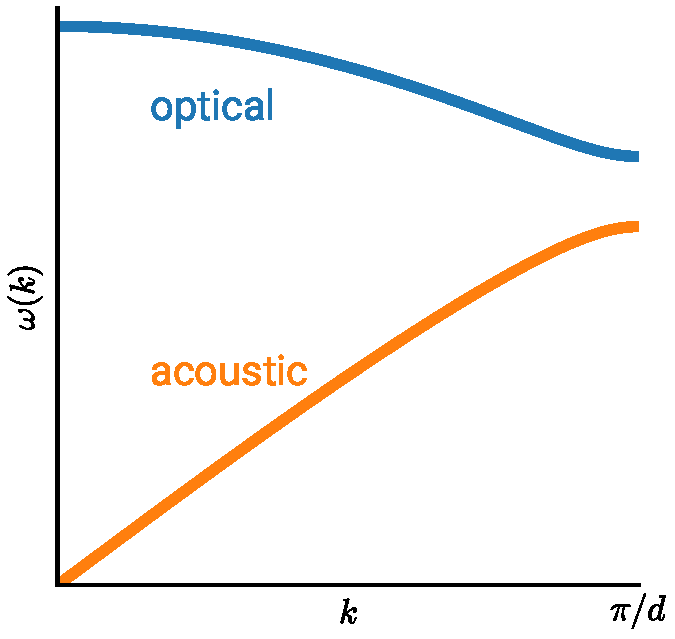
\includegraphics[width=0.5\linewidth]{phonon-modes.pdf} \label{phonon-modes}} \hspace{3ex}
	\subfloat[]{\includegraphics[width=0.37\linewidth]{phonon-absorption.png} \label{phonon-absorption}}
	\caption{\protect\subref{phonon-modes} Dispersion relation for phonons in a solid with two atoms per unit cell. The acoustic mode governs thermomechanical properties while the optical mode governs electronic properties. \protect\subref{phonon-absorption} Transmissivity of a film of RbI at different temperatures, with each minimum at a photon energy equal to that of the long wavelength transverse optical phonon. Reproduced from G. O. Jones et al. \href{http://rspa.royalsocietypublishing.org/content/261/1304/10}{\emph{Proc. R. Soc. London}} A261, 1961.}
	\label{fig:phonon-modes}
\end{figure}

When atoms are vibrating coherently (in the same direction; corresponding to the minus sign in the above equation), \textbf{acoustic phonons} are produced, named because they modulate the speed of sound in the medium as well as the medium's mechanical and thermal properties.\footnote{See A. A. Balandin \href{https://www.nature.com/nmat/journal/v10/n8/full/nmat3064.html}{\emph{Nat. Mater.}} 10, 2011, for a review of the thermal properties of carbon nanostructures.} 
On the other hand, atoms vibrating out-of-phase (in opposite directions) will produce \textbf{optical phonons}, which interact with light in absorption and \emph{Raman scattering}. 


% % % % % % % % % % % % % % % % % % % % % % % % % % % % % % % % % % % % % 
% % % % % % % % % % % % % % % % % % % % % % % % % % % % % % % % % % % % %
% % % % % % % % % % % % % % % % % % % % % % % % % % % % % % % % % % % % %
\section{Summary}

To recap, this chapter gave us a taste of quantum field theory and some of its important applications. 
Second quantization provided a suitable framework for interpreting fields with the new occupation number operator and new definitions for the creation and annihilation operators. 
Then we explored the strange nature of the Casimir effect using regularization and renormalization to handle various infinities. 
Finally, we related the theoretical framework of QFT to phonons, which are quantized lattice vibrations that govern a lot of material behavior. 
This chapter was largely enrichment in the context of this course, but you will definitely see more of QFT as you take more advanced courses in quantum mechanics due to its profound implications. 
Perturbation theory, which we will see in the next chapter, is another subfield of quantum mechanics that shares similarities with QFT.

%} % for doublespacing
%\end{document}